\chapter{Spectral Emissivity Library of Spoil Substrates}
\label{app:Library}

The spectral library consists of 24 ASCII files. Each file describes one spoil substrate. Individual files are named according to the sample number. Files consist of a file header and spectral emissivities. Both file parts are described in the subsections below.

\section{Header}

The format of header is similar to format of ASTER Spectral Library header \cite{BH09}. Each file contains 26 lines of header, which includes available sample information. The header is divided into four sections separated by empty lines. First part contains 9 lines discussing sample classification, particle size and sample origin. Sample origin is expressed by latitude and longitude on the reference ellipsoid WGS84. This information is summarized in the following fields:

\begin{enumerate}
	\item	Name
	\item Type
	\item Class
	\item Particle size
	\item Sample No
	\item Owner
	\item Origin
	\item Latitude
	\item Longitude
\end{enumerate}

A second section contains information about sample toxicity and chemical properties. The unit of each quantity is indicated in square brackets after quantity name. This header section contains following fields:

\begin{enumerate}
	\item toxicity
	\item pH in H20
	\item pH in KCl
	\item conductivity
	\item water soluble Na
	\item water soluble K
	\item Al in KCl
	\item Fe in KCl
	\item loss on ignition
	\item polyphenol content
\end{enumerate}

A third section contains reference to \cite{FK05}, which discusses toxicity measurement and chemical analysis. Finally, the fourth header section contains the names of two columns, in which the following spectral emissivity data are aligned. Metadata in each header line contains an attribute name followed by a colon (ASCII Character 3A) and tab (ASCII Character 09) and then the corresponding value.

\section{Spectral Emissivity}

After the header part, the file continues on lines 27 – 213 with spectral emissivity data aligned in two columns. As header file indicates, the first column contains wavelength in micrometers and the second column contains corresponding emissivity value. Values in each row are separated by tab. The emissivity of each sample is provided in wavelengths interval from 8 µm to 14 µm. Sampling in this interval is non-linear.

\begin{figure*}[!t]
\centering
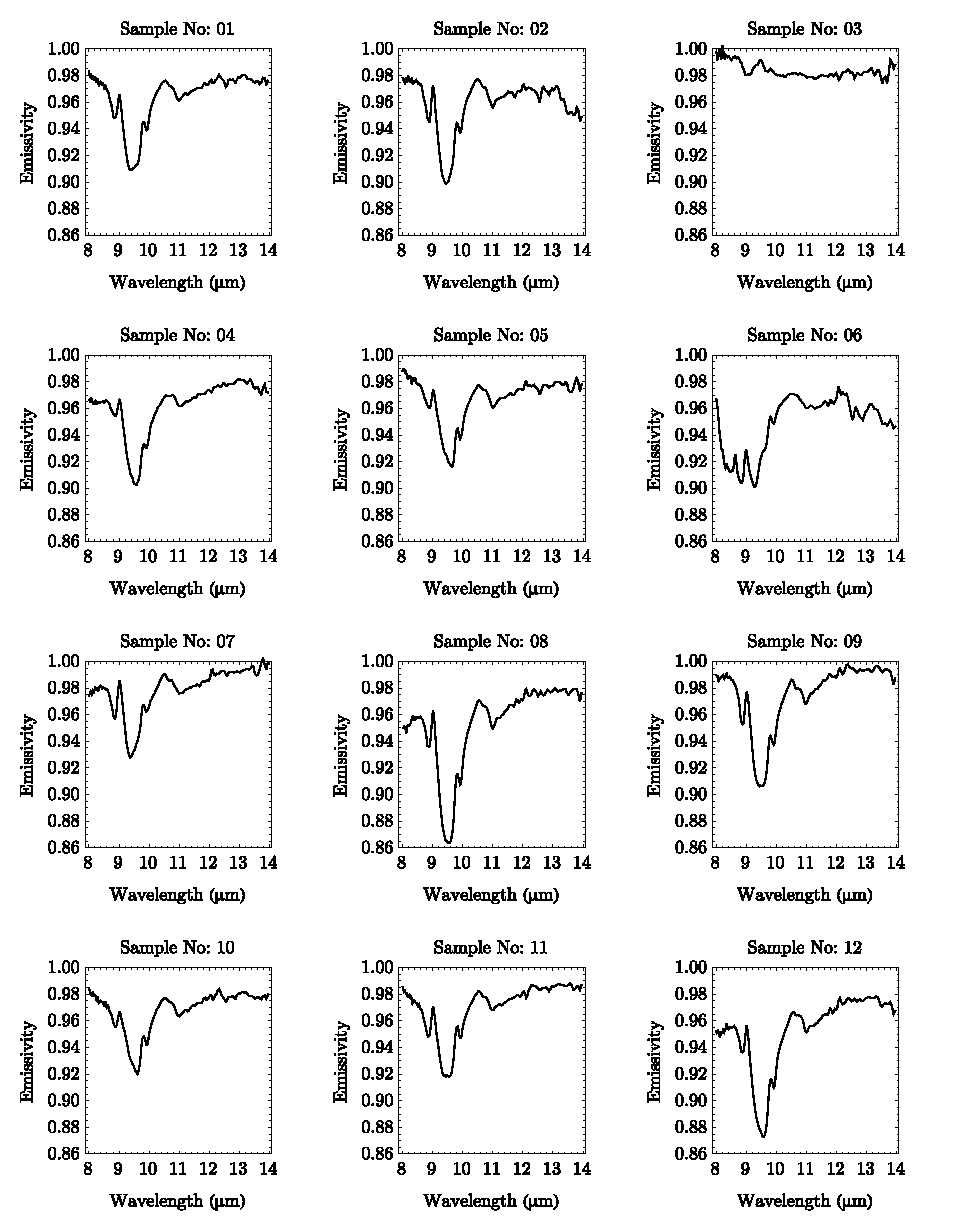
\includegraphics[width=0.95\linewidth]{pics/Chapter_05/spectral_library_pt1.eps}
\vspace{1.5 em}
\caption{TODO.}
\label{fig:SpoilSubstratesPreviewPt1}
\end{figure*}

\begin{figure*}[!t]
\centering
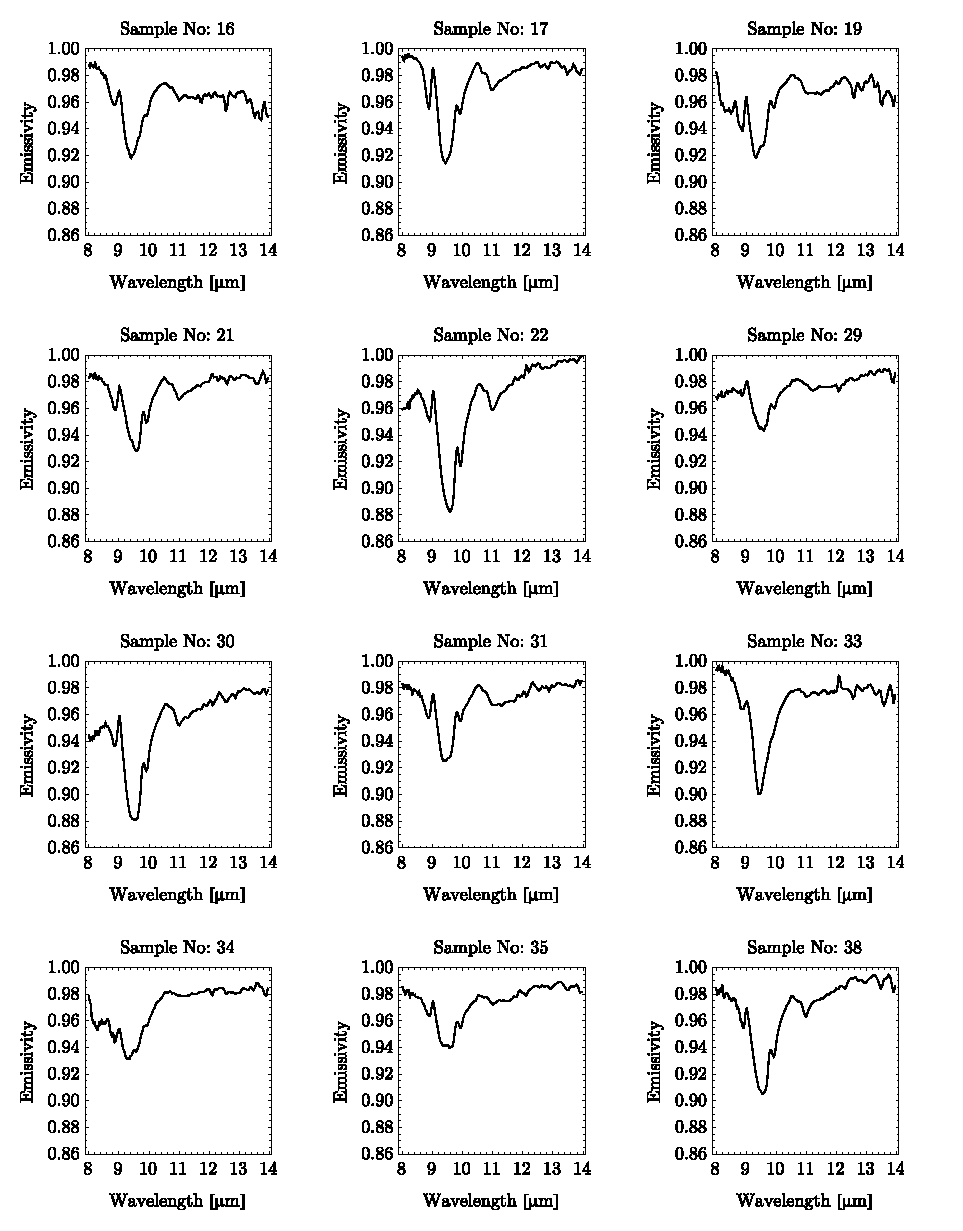
\includegraphics[width=0.95\linewidth]{pics/Chapter_05/spectral_library_pt2.eps}
\vspace{1.5 em}
\caption{TODO.}
\label{fig:SpoilSubstratesPreviewPt1}
\end{figure*}

\end{appendices}